The CPU datapath is shown in figure \ref{fig:datapath}. It is highly
configurable as to allow for adding new instructions with ease. Because of the
datapath's structure, instructions can be multiple cycles. It should be
mentioned that the memory module is not part of the datapath, but shown in the
figure for clarity.\par
The accumulator register is labelled \texttt{ac} in the figure, and as shown,
can be selectively loaded from one of four sources. The Arithmetic Logic Unit,
\texttt{alu0}, is capable of performing a total of eight operations, with or
without the use of the flags register. The microcode (section
\ref{subsec:microcode_rom}) is programmed so that every ALU operation stores a
new set of flags in the flags register, \texttt{flags}. The second operand to
the ALU can be chosen from a total of 8, allowing for maximum
configurability.\par
The memory subsystem in the datapath allows for both direct and indirect
addressing, with two sources for the memory address register \texttt{mar}. Data
sources for memory on the \texttt{mdr} register can be chosen from a total of
4, allowing further configuration options.\par
For ease of implementation, the program counter subsystem was also added to the
datapath. To save instruction execution time, an extra adder was included to
compute the next sequential execution address, rather than use the existing
ALU. This also allows for the next program counter address to be stored on the
program counter register, \texttt{pc}, on the last microinstruction of the
currently executing instruction (see section \ref{subsec:microcode_rom}). The
program counter subsystem allows for direct branching, indirect branching and
relative branching as well as the regular execution flow.
\begin{figure}[h]
	\centering
	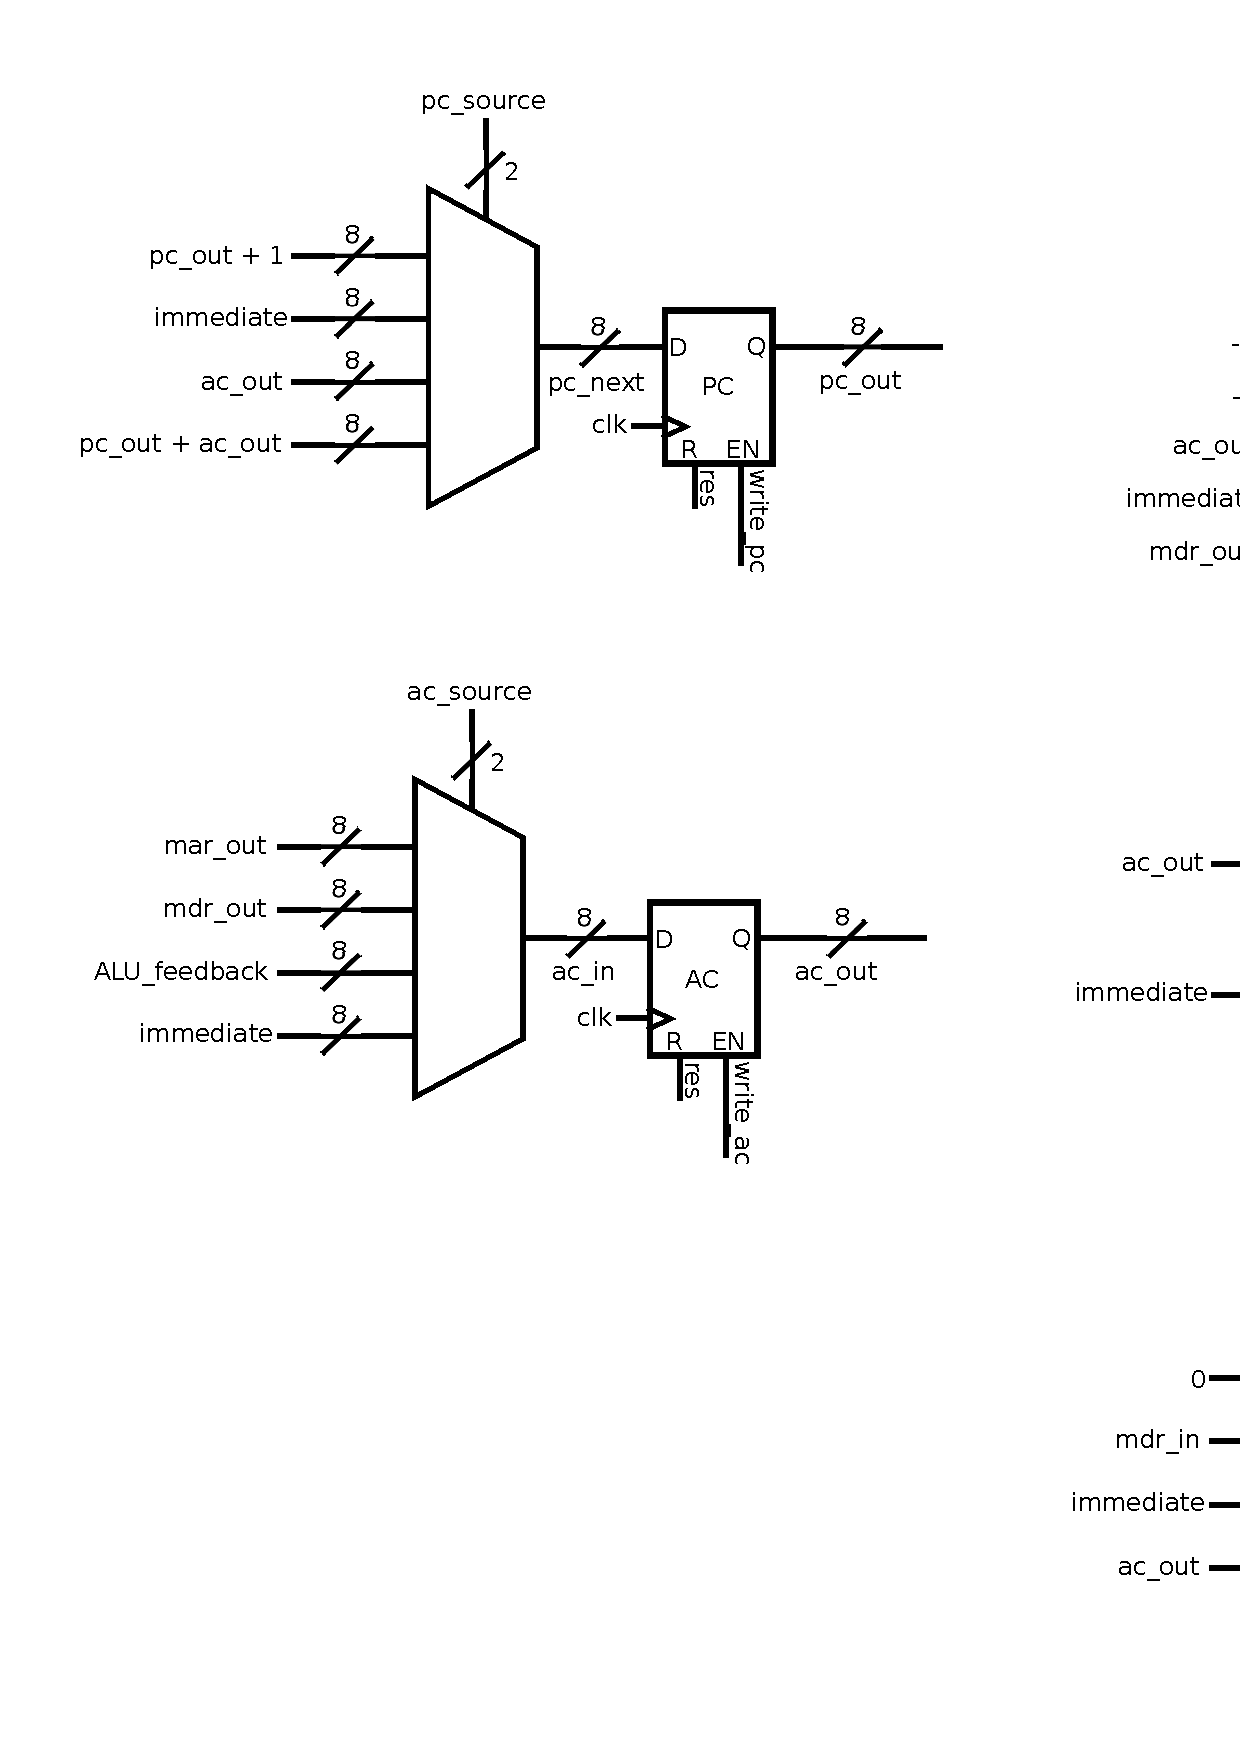
\includegraphics[width=\textwidth]{../fig/datapath.pdf}
	\caption{CPU datapath module structure}
	\label{fig:datapath}
\end{figure}
